% Shared body. Build conecct.tex (anonymous, double-blind) or arxiv.tex (named authors).
\documentclass[conference]{IEEEtran}
\IEEEoverridecommandlockouts
\usepackage{cite}
\usepackage{amsmath,amssymb}
\usepackage{graphicx}
\usepackage{booktabs}
\usepackage{url}
\usepackage{tikz}
\usepackage{algorithm}
\usepackage{algpseudocode}
\usetikzlibrary{positioning,arrows.meta}
\usepackage[hidelinks]{hyperref}

\providecommand{\anonymous}{1}
\newcommand{\coderef}{\ifnum\anonymous=1 [repository link withheld for double-blind review]\else \url{https://github.com/rushikbuilds/ML-Drift-Monitoring-System}\fi}

\begin{document}

\title{Early Warning of Model Degradation under Delayed Labels:\\ A Pre-Registered Evaluation of Drift and Harm Signals}

\ifnum\anonymous=1
\author{\IEEEauthorblockN{Anonymous Authors}
\IEEEauthorblockA{Affiliation withheld for double-blind review}}
\else
% IEEE style: plain names (no titles or roles), one shared affiliation block.
% TODO: replace [Department ...] and the e-mail placeholders before submission.
\author{\IEEEauthorblockN{Akshay Naphade, Rushikesh Kadepurkar, Parth Tatpuje, Vishnu Gurav and Sunil Bhirud}
\IEEEauthorblockA{\textit{[Department of ...]}, \textit{COEP Technological University}, Pune, India\\
\{[akshay-email], [rushikesh-email], [parth-email], [vishnu-email], [guide-email]\}@[domain]}}
\fi

\maketitle

\begin{abstract}
Deployed classifiers often lose accuracy long before true labels arrive to reveal it. Drift detectors offer earlier signals, but most input shifts do not harm the model, and thresholds tuned on one dataset may not hold on another. We built a two-tier early-warning monitor and evaluated it with pre-registered hypotheses, frozen thresholds and one-time runs on datasets never used during design. Streams are built by re-sampling real rows so that inputs drift from a known batch while every row keeps its true label, which lets us measure harm instead of assuming it. A first design, a learned risk calibrator over raw drift scores, failed all five pre-registered hypotheses: thresholds in raw units did not transfer, and false alerts on unseen datasets ranged from 1.2 to 44.6 per 100 clean batches against a budget of 5. Expressing every signal relative to the stream's own burn-in period fixed this. The resulting drift-watch tier warned before the accuracy drop on 87\% of harmful gradual shifts, a median of six batches ahead, at 4.4 false alerts per 100 clean batches. A second tier that estimates accuracy from an importance-weighted labeled reference cut alarms on harmless shifts from 97\% to 34\% and separated harmful from harmless shifts with an AUROC of 0.78 (95\% CI 0.70--0.86), just below our pre-registered 0.80 target. More flexible estimators, ensembles and stricter alerting rules did not improve on it on fresh data. We release the benchmark, code and all verdicts.
\end{abstract}

\begin{IEEEkeywords}
concept drift, dataset shift, model monitoring, delayed labels, performance estimation, pre-registration, MLOps
\end{IEEEkeywords}

\section{Introduction}
A classifier is trained on past data and deployed on a stream whose distribution changes. Whether the change hurts is known only once true labels arrive, which in credit, fraud or churn prediction can take days or weeks. Monitoring systems therefore watch label-free signals such as feature distributions and prediction confidence~\cite{sculley2015debt,breck2017mltest}. Two practical problems limit them. First, most distribution shifts are harmless to a given model~\cite{rabanser2019failing}, so drift alarms fire on changes that do not matter. Second, alarm thresholds are usually chosen on historical data, and it is rarely tested whether they still mean the same thing on a new dataset.

We study a monitor that should warn about \emph{degradation}, not merely drift, before delayed labels confirm it. We report what worked and what did not, and we constrained ourselves to make that report trustworthy: every hypothesis, pass threshold and alert threshold was frozen in code before the data that judged it existed, every confirmation used datasets not touched during design, and a script computed each verdict.

Our contributions are:
\begin{enumerate}
\item A benchmark that re-samples real tabular data to create gradual, abrupt and irrelevant-feature shifts and label changes with a known onset, where whether a shift harms the model is measured from true labels.
\item Evidence that drift thresholds expressed in raw units do not transfer across datasets, and that expressing signals relative to a stream's own burn-in period does: an early drift warning that holds its false-alert budget on unseen data.
\item A label-free harm tier based on importance-weighted reference accuracy that substantially reduces alarms on harmless shifts, with an honest account of where it falls short.
\item Pre-registered negative results, including three follow-up attempts to exceed the harm-separation target that failed on fresh data.
\end{enumerate}

\section{Related Work}
\textbf{Concept drift.} Surveys cover detection and adaptation under drift~\cite{gama2014survey,lu2019review}. Classical detectors such as DDM~\cite{gama2004ddm} and ADWIN~\cite{bifet2007adwin} monitor the error stream and therefore need labels; sequential tests such as CUSUM~\cite{page1954cusum} accumulate evidence of a persistent change. Label-free detection compares feature or embedding distributions with two-sample tests such as Kolmogorov--Smirnov or maximum mean discrepancy~\cite{gretton2012mmd}; Rabanser et al.~\cite{rabanser2019failing} evaluated such detectors and noted that detected shift need not reduce accuracy. Dataset shift and label shift are treated in~\cite{quinonero2009shift,lipton2018labelshift}.

\textbf{Label-free performance estimation.} Confidence-based estimation (CBPE)~\cite{nannyml_cbpe}, average thresholded confidence~\cite{garg2022atc}, difference of confidences~\cite{guillory2021doc} and model disagreement~\cite{jiang2022disagreement} estimate accuracy without labels. Under covariate shift, importance weighting reweights source samples by the density ratio~\cite{shimodaira2000,sugiyama2007iwcv}; we use it to estimate the frozen model's accuracy on each batch from a labeled reference set.

\textbf{Delayed labels.} Learning and evaluation when labels arrive late or never are studied in~\cite{grzenda2020delayed,umer2020evl}. We use a fixed delay of $L$ batches and ask how early a monitor can warn relative to the moment delayed labels could confirm a drop.

\textbf{Pre-registration.} Fixing hypotheses and analysis before seeing results reduces analytic flexibility~\cite{vanmiltenburg2021prereg}; we apply it to an ML monitoring evaluation, including thresholds.

\section{Problem Setting and Protocol}
A frozen binary classifier $f$ is trained on a labeled reference set $R$ and then scores a stream of batches $B_1, B_2, \dots$ of 300 rows. The labels of batch $b$ become usable at batch $b+\max(L,1)$, with label delay $L$ (primary setting $L=5$). The first 8 batches after deployment form a burn-in period during which no alerts are raised.

\textbf{Degradation event.} The baseline is the mean accuracy of batches 0--4. An event begins at the first of two consecutive batches whose accuracy is at least 5 points below the baseline.

\textbf{Warning tiers.} For an intervention starting at batch $s$ and an event at batch $e$, a \emph{predictive warning} (T1) is an alert in $[s, e)$, and a \emph{pre-confirmation warning} (T2) is an alert in $[s, e+1+\max(L,1))$, i.e., before delayed labels could confirm the event.

\textbf{False alerts.} Clean batches are the batches of unshifted streams and the pre-shift batches of every other stream. The budget is 5 false alerts per 100 clean batches. For shifts that cause no event (harmless shifts) we report the share of episodes with any alert after onset.

\textbf{Pre-registration.} For each experiment we committed, before obtaining its confirmation data, a configuration module defining datasets, seeds, the method, the threshold rule and each hypothesis with its pass rule. Thresholds were chosen on development data only and frozen with recorded SHA-256 fingerprints; the confirmation script refuses to run if they change. Deviations (for example, shuffling a dataset whose rows are stored sorted by class) were logged with date and reason before any affected episode was built.

\section{Benchmark}
Each episode draws a contiguous block of a dataset: 2000 reference rows (1500 to fit $f$, 500 held out to compute its permutation feature importance) and a pool of the next 20,000 rows. Because the reference and the pool come from one period, an unshifted stream has no built-in drift. The stream has 45 batches sampled with replacement from the pool; every row keeps its true label. From an onset batch $s \in [10, 16]$:
\begin{itemize}
\item \emph{gradual / abrupt shift}: rows are sampled with weights $\propto \exp(\lambda(t)\, \sigma\, z_j)$, where $z_j$ is a standardized feature, $\sigma=\pm1$, and $\lambda$ ramps to 1.5 over 15 batches (gradual) or jumps to 1.5 (abrupt). The feature is drawn from the more or the less important half with equal probability;
\item \emph{label change}: labels are flipped with a probability ramping to 0.3 for rows with $z_k>0$;
\item \emph{clean}: uniform sampling.
\end{itemize}
Algorithm~\ref{alg:episode} summarizes the construction. Each dataset contributes 10 clean, 30 gradual, 15 abrupt and 10 label-change episodes.

\begin{algorithm}[t]
\caption{Building one benchmark episode}
\label{alg:episode}
\footnotesize
\begin{algorithmic}[1]
\Require dataset $(X, y)$, kind, seed
\State draw a block start where both classes are $\geq$5\% of the fit rows and the pool
\State $R \gets$ next 2000 rows; fit $f$ on the first 1500, importance on the last 500
\State $P \gets$ next 20{,}000 rows (pool); draw onset $s \in [10,16]$
\If{kind is a shift} \State pick feature $j$ (important or unimportant half), sign $\sigma$ \EndIf
\For{$t = 0, \dots, 44$}
  \If{kind is a shift and $t \geq s$}
    \State sample 300 rows of $P$ with weights $\propto \exp(\lambda(t)\,\sigma\, z_j)$
  \Else
    \State sample 300 rows of $P$ uniformly
  \EndIf
  \If{kind is a label change and $t \geq s$} \State flip labels of rows with $z_k > 0$ w.p. $0.3\,\min(1, (t-s+1)/15)$ \EndIf
\EndFor
\State measure accuracy of $f$ per batch; label the episode harmful, harmless or clean by the event rule
\end{algorithmic}
\end{algorithm} A shift episode is \emph{harmful} if its event starts after onset and \emph{harmless} if no event occurs; episodes with an event before onset are excluded. Across all data groups only about one shift in five was harmful, and harm was barely related to the importance of the shifted feature; it did not change when the shift strength $\lambda$ was raised from 1.5 to 4.0.

Datasets come from OpenML~\cite{vanschoren2014openml}. The first study (v6) used 13 datasets, 8 for development (covertype, CovPokElec, Hyperplane, KDDCup99, LED, poker-hand, run-or-walk, vehicle-SensIT) and 5 held out (airlines, bank-marketing, electricity, ldpa, SEA). Later confirmations used fresh datasets: adult, MiniBooNE, higgs, nomao, numerai28.6 and Click-prediction-small (v7); default-of-credit-card-clients, kick, house-16H, 2dplanes and mv (v8). The primary model is logistic regression~\cite{pedregosa2011sklearn}; gradient boosting was a robustness check in v6. Table~\ref{tab:data} summarizes how the data were used; each group served exactly one purpose, and confirmation groups were downloaded only after the corresponding design and thresholds were frozen.

\begin{table}[t]
\caption{Data groups and their single use (65 episodes per dataset).}
\label{tab:data}
\centering
\footnotesize
\begin{tabular}{@{}lcl@{}}
\toprule
Group & Datasets & Use \\
\midrule
v6 development & 8 & design, thresholds, all later tuning \\
v6 held-out & 5 & one-time v6 verdict \\
v7 confirmation & 6 & one-time drift-watch verdict \\
v8 confirmation & 5 & one-time harm-tier verdict \\
v10 confirmation & 6 & one-time test of alerting rules \\
Natural streams & 13 & H5/C5 (no injected shift) \\
\bottomrule
\end{tabular}
\end{table}

\section{Monitoring Methods}
Fig.~\ref{fig:system} summarizes the final two-tier design: both warning tiers use only label-free signals and the labeled reference set, and delayed labels later confirm or clear a warning.

\begin{figure}[t]
\centering
\resizebox{\columnwidth}{!}{%
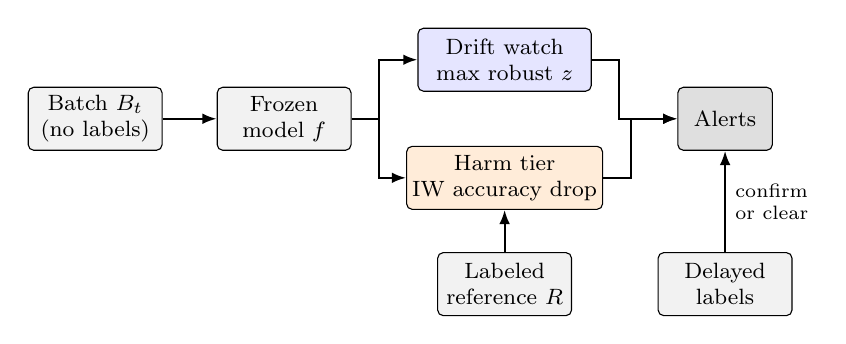
\begin{tikzpicture}[font=\footnotesize,
  box/.style={draw, rounded corners=2pt, align=center, minimum height=8mm, minimum width=17mm, inner sep=2pt},
  arr/.style={-{Latex[length=1.8mm]}, thick}]
\node[box, fill=gray!10] (stream) at (0,0) {Batch $B_t$\\(no labels)};
\node[box, fill=gray!10] (model) at (2.4,0) {Frozen\\model $f$};
\node[box, fill=blue!10, minimum width=22mm] (watch) at (5.2,0.75) {Drift watch\\max robust $z$};
\node[box, fill=orange!15, minimum width=22mm] (harm) at (5.2,-0.75) {Harm tier\\IW accuracy drop};
\node[box, fill=gray!10] (ref) at (5.2,-2.1) {Labeled\\reference $R$};
\node[box, fill=gray!25, minimum width=12mm] (alert) at (8.0,0) {Alerts};
\node[box, fill=gray!10] (labels) at (8.0,-2.1) {Delayed\\labels};
\draw[arr] (stream) -- (model);
\draw[arr] (model.east) -- ++(0.35,0) |- (watch.west);
\draw[arr] (model.east) -- ++(0.35,0) |- (harm.west);
\draw[arr] (ref) -- (harm);
\draw[arr] (watch.east) -- ++(0.35,0) |- (alert.west);
\draw[arr] (harm.east) -- ++(0.35,0) |- (alert.west);
\draw[arr] (labels) -- node[right, align=left, font=\scriptsize]{confirm\\or clear} (alert);
\end{tikzpicture}}
\caption{Two-tier early-warning monitor. The drift watch flags changes in inputs or model behavior; the harm tier estimates whether accuracy is falling; delayed labels confirm or clear the warning.}
\label{fig:system}
\end{figure}

\textbf{Signals.} Per batch the monitor computes, without labels: a fused drift score combining per-feature statistics (KS, PSI) with an embedding MMD and a confidence component; the mean KS statistic; a relevance-weighted shift (KS weighted by the model's permutation importance); disagreement between $f$ and two auxiliary models trained on the same reference rows; mean confidence and entropy; and the shift in the positive-prediction rate.

\textbf{v6: learned risk calibrator.} A logistic model maps these raw signals, their recent means and slopes, and the observed accuracy drop from matured labels to the probability that a degradation starts or continues within 5 batches. Thresholds are chosen on development data to maximize T1 within the false-alert budget.

\textbf{v7: drift watch (stream-normalized).} Each signal $x_t$ is converted to a robust z-score using the burn-in, $z_t = (x_t - \mathrm{med}(x_{0:8})) / \max(1.4826\,\mathrm{MAD}(x_{0:8}), 0.01)$, and the drift-watch score is the maximum z-score over seven label-free signals. A threshold of 4.0 deviations, chosen on development data, means the same thing on every stream.

\textbf{v8: harm tier.} For each batch $B_t$, a logistic domain classifier $g_t$ is trained to separate reference rows (label 0) from batch rows (label 1). For reference row $x_i$ with correctness $c_i = \mathbb{1}[f(x_i)=y_i]$, the importance weight and the label-free accuracy estimate are
\begin{equation}
w_i = \min\!\left(\frac{\rho_i}{\bar\rho}, 20\right),\quad \rho_i=\frac{g_t(x_i)}{1-g_t(x_i)},\qquad \hat a_t = \frac{\sum_i w_i c_i}{\sum_i w_i},
\end{equation}
where $\bar\rho$ is the mean odds over the reference. Under covariate shift, $\hat a_t$ targets the accuracy of $f$ on $B_t$~\cite{shimodaira2000,sugiyama2007iwcv}. The harm score is $h_t = \mathrm{med}(\hat a_{0:8}) - \hat a_t$, the estimated drop in accuracy points since the burn-in. Its threshold (an estimated drop of 1.15 points) was chosen on development data to maximize T2 on harmful shifts minus the alert share on harmless shifts, within the budget.

\section{Results}
All results use logistic regression and label delay $L=5$. Intervals are 95\% bootstrap intervals over episodes.

\subsection{v6: the original design fails}
Table~\ref{tab:v6} shows the pre-registered verdict on the 5 held-out datasets (53 harmful and 169 harmless shifts). The learned calibrator warned before the drop on only 22\% of harmful gradual shifts and did not beat waiting for delayed labels. The fused drift score's higher warning rates came from alerting almost constantly. Among the secondary settings (Table~\ref{tab:scarce}), the gradient-boosting system warned before confirmation more often than the delayed-label trend when only 20\% of rows were ever labeled, but its false alerts exceeded the budget at most delays, and the logistic system stayed below the label trend; we therefore make no claim from these settings.


\begin{table}[t]
\caption{v6 pre-registered hypotheses on held-out datasets.}
\label{tab:v6}
\centering
\footnotesize
\begin{tabular}{@{}p{3.55cm}p{2.75cm}l@{}}
\toprule
Hypothesis (target) & Result & Verdict \\
\midrule
H1: T1, harmful gradual ($\geq$0.60) & 0.22 [0.08, 0.36] & Fail \\
H2: T2 gain vs labels ($\geq$0.10) & $-$0.02 [$-$0.11, 0.08] & Fail \\
H3: harm AUROC ($\geq$0.80); harmless alerts ($\leq$0.10) & 0.59; 0.37 & Fail \\
H4: beats fused drift score ($\geq$4 of 5 datasets) & 2 of 5 & Fail \\
H5: natural streams, T2 gain ($\geq$0) & $-$0.01 [$-$0.08, 0.06] & Fail \\
\bottomrule
\end{tabular}
\end{table}
\begin{table}[t]
\caption{v6 secondary settings with 20\% of labels (held-out): T2 on harmful shifts, and false alerts per 100 clean batches.}
\label{tab:scarce}
\centering
\footnotesize
\setlength{\tabcolsep}{4pt}
\begin{tabular}{@{}lcccc@{}}
\toprule
Model, delay & Sys.\ T2 & Labels T2 & Sys.\ FA & Labels FA \\
\midrule
Logistic, $L{=}0$ & 0.43 & 0.58 & 1.7 & 4.5 \\
Logistic, $L{=}5$ & 0.49 & 0.70 & 1.0 & 5.0 \\
Grad.\ boosting, $L{=}0$ & 0.64 & 0.48 & 3.9 & 4.0 \\
Grad.\ boosting, $L{=}2$ & 0.73 & 0.57 & 5.7 & 5.1 \\
Grad.\ boosting, $L{=}5$ & 0.73 & 0.61 & 5.3 & 4.9 \\
Grad.\ boosting, $L{=}10$ & 0.82 & 0.80 & 7.7 & 5.9 \\
\bottomrule
\end{tabular}
\end{table}

\subsection{Why: thresholds in raw units do not transfer}
Fig.~\ref{fig:transfer} compares false-alert rates on development data with those on data never used for threshold selection. Scores in dataset-specific units broke the budget by a factor of 3.5--9 (fused drift score 4.4~$\rightarrow$~36.9; mean KS 4.4~$\rightarrow$~44.6), while the learned calibrator under-alerted (4.6~$\rightarrow$~1.2). Scores expressed relative to the stream's own normal (drift watch, 2.3~$\rightarrow$~4.4) or in accuracy points (harm tier, 3.4~$\rightarrow$~2.8) stayed within the budget. An ablation confirmed the mechanism inside the calibrator: removing the raw disagreement levels, which differ widely across datasets, raised its T1 from 0.22 to 0.42.

\begin{figure}[t]
\centering
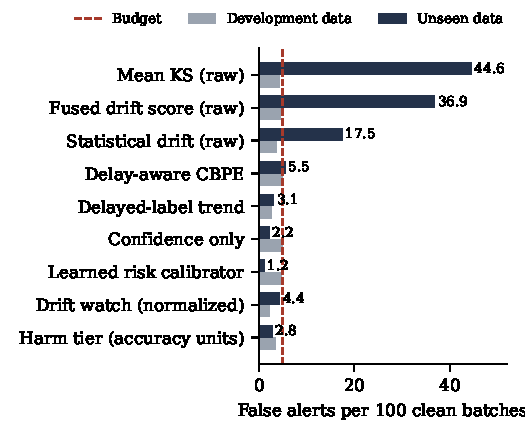
\includegraphics[width=\columnwidth]{figures/transfer.pdf}
\caption{False alerts per 100 clean batches with thresholds chosen on development data, evaluated on development and on unseen datasets. Dashed line: budget of 5.}
\label{fig:transfer}
\end{figure}

\subsection{v7: the drift watch tier}
On six fresh datasets (39 harmful gradual shifts) the drift watch warned before the accuracy drop on 0.87 [0.77, 0.97] of harmful gradual shifts, a median of 6 batches ahead, with 4.4 false alerts per 100 clean batches, and beat the fused drift score on 5 of 6 datasets (Table~\ref{tab:confirm}). Its pre-confirmation warning rate (1.00 vs 0.96 for the delayed-label trend) did not reach the pre-registered gain of 0.10. It alerted on 96\% of harmless shifts: it is a drift detector, not a harm detector. On natural streams it failed (T2 0.44 vs 0.87 for the label trend): there, the median degradation began at batch 8, the end of the burn-in, so the burn-in did not represent normal behavior. The v7 verdict was a partial success.

\subsection{v8: the harm tier}
On five further fresh datasets (64 harmful and 160 harmless shifts), the harm tier cut alarms on harmless shifts from 0.97 (drift watch) to 0.34 while still warning before labels could confirm on 0.83 of harmful shifts and before the drop on 0.76 of harmful gradual shifts, at 2.8 false alerts per 100 clean batches. It separated harmful from harmless shifts with an AUROC of 0.78 [0.70, 0.86], against 0.59 for the drift watch (gain 0.20 [0.09, 0.30]). It passed two of four hypotheses and missed the AUROC target of 0.80 and the harmless-alarm target of 0.10. Per dataset (Table~\ref{tab:perds}), the harm tier separated harm well on three of the four datasets that produced harmful shifts and was near chance on kick. Fig.~\ref{fig:timeline} shows one harmful gradual shift: the harm tier first alerts at batch 16, 14 batches before the accuracy drop and 20 before delayed labels confirm it.

\begin{table}[t]
\caption{Confirmation on fresh datasets (one-time runs).}
\label{tab:confirm}
\centering
\footnotesize
\begin{tabular}{@{}lcc@{}}
\toprule
& v7 drift watch & v8 harm tier \\
\midrule
Datasets & 6 & 5 \\
T1, harmful gradual shifts & 0.87 & 0.76 \\
T2, harmful shifts & 1.00 & 0.83 \\
False alerts / 100 clean batches & 4.4 & 2.8 \\
Harmless shifts with an alert & 0.96 & 0.34 \\
Harm AUROC & 0.51 & 0.78 \\
Pre-registered verdict & partial success & partial success \\
\bottomrule
\end{tabular}
\end{table}

\begin{table}[t]
\caption{Harmful-vs-harmless AUROC per v8 confirmation dataset.}
\label{tab:perds}
\centering
\footnotesize
\begin{tabular}{@{}lcccc@{}}
\toprule
Dataset & Harmful & Harmless & Harm tier & Drift watch \\
\midrule
2dplanes & 14 & 31 & 0.98 & 0.64 \\
credit default & 8 & 36 & 0.89 & 0.58 \\
house-16H & 26 & 19 & 0.78 & 0.60 \\
kick & 16 & 29 & 0.61 & 0.60 \\
mv & 0 & 45 & -- & -- \\
\bottomrule
\end{tabular}
\end{table}

\begin{figure}[t]
\centering
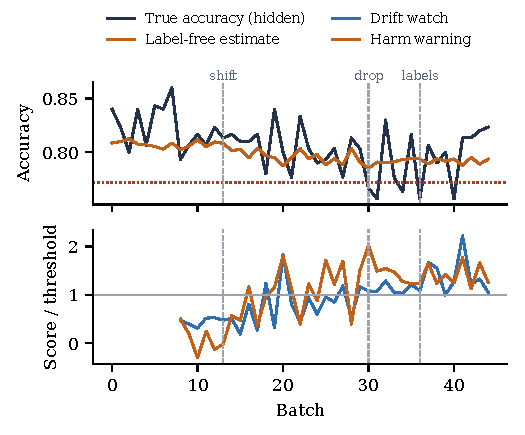
\includegraphics[width=\columnwidth]{figures/timeline.pdf}
\caption{A harmful gradual shift on an unseen dataset (credit default, $L=5$). Top: true accuracy (hidden from the monitor) and the label-free estimate; dotted line: 5 points below baseline. Bottom: tier scores divided by their thresholds; above 1 is an alert.}
\label{fig:timeline}
\end{figure}

\subsection{Why harmless shifts still alert}
In a post-hoc analysis of the v8 confirmation data, streams with no shift at all raised a harm alert in 40\% of episodes and harmless shifts in 34\%, against 88\% for harmful shifts. The harm tier therefore treats harmless shifts like no shift; the remaining alarms are background false alerts that accumulate over about 33 monitored batches. With a per-batch rate of 2.8 per 100, the chance of at least one alert in 33 batches is about 0.6. Our 10\% target was inconsistent with our own per-batch budget, a design error we report rather than correct after the fact.

Fig.~\ref{fig:operating} shows the full trade-off on the same data, post hoc. At every level of harmless alarms the harm tier warns on far more harmful shifts than the drift watch. On this data a stricter harm threshold would appear better than the frozen one, but when that idea was frozen and tested on six other datasets (v10, square marker) it warned on only 30\% of harmful shifts: an operating point read off a curve after the fact does not transfer.

\begin{figure}[t]
\centering
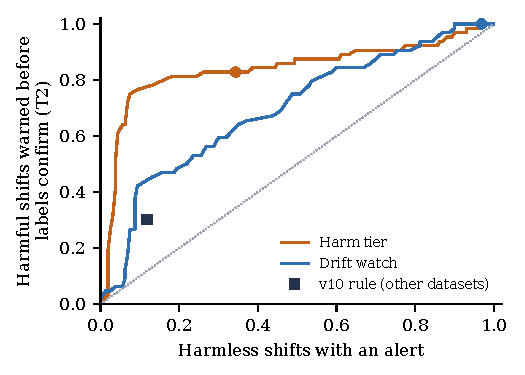
\includegraphics[width=\columnwidth]{figures/operating.pdf}
\caption{Post hoc operating curves on the v8 confirmation data: each point is a threshold. Circles: frozen thresholds. Square: the stricter v10 rule, frozen on development data and evaluated on six different datasets.}
\label{fig:operating}
\end{figure}

\subsection{Pre-registered follow-ups that failed}
Two further experiments tried to improve the harm tier (Table~\ref{tab:followups}). In v9, a gradient-boosting domain classifier and an error predictor trained on out-of-fold reference correctness both separated harm worse than the linear estimator on development data (AUROC 0.70 vs 0.77), as did every ensemble of the estimators (at most 0.76); the development gate of 0.80 failed and no fresh data were used. In v10, stricter thresholds, smoothing, CUSUM, stream-normalized scores and gating by the drift watch all reduced harmless alarms at the cost of early warnings. The best rule passed the development gate but, on six fresh datasets, warned before labels on only 0.30 of harmful shifts against a required 0.50, while reducing harmless alarms to 0.12. Neither was adopted.

\begin{table}[t]
\caption{Follow-up experiments (not adopted).}
\label{tab:followups}
\centering
\footnotesize
\begin{tabular}{@{}p{3.1cm}p{4.6cm}@{}}
\toprule
Attempt & Outcome \\
\midrule
v9: nonlinear harm estimators, ensembles & Development AUROC 0.70 (vs 0.77); ensembles $\leq$0.76; gate failed \\
v10: stricter alerting rules & Fresh data: harmless 0.12 but T2 0.30 ($<$0.50); confirmation failed \\
\bottomrule
\end{tabular}
\end{table}

\section{Discussion and Limitations}
\textbf{Units matter more than models.} The decisive change between the failed and the partially successful designs was not a better model but expressing signals in units that mean the same thing on every stream. Monitoring thresholds tuned on historical data should be validated on data from other sources before deployment.

\textbf{Drift and harm need different signals.} Using each normalized signal alone as the drift watch on the v7 confirmation data (Table~\ref{tab:signals}), input-shift signals warned early on 79--90\% of harmful gradual shifts but could not tell harm from harmlessness (AUROC about 0.5), whereas model-behavior signals were harm-aware (AUROC 0.72--0.77) but warned later.

\begin{table}[t]
\caption{Each normalized signal used alone (v7 confirmation data, post hoc).}
\label{tab:signals}
\centering
\footnotesize
\setlength{\tabcolsep}{4pt}
\begin{tabular}{@{}llccc@{}}
\toprule
Family & Signal & T1 & Harmless & AUROC \\
\midrule
Input shift & fused drift score & 0.90 & 0.95 & 0.52 \\
 & mean KS & 0.90 & 0.95 & 0.53 \\
 & relevance-weighted shift & 0.79 & 0.92 & 0.51 \\
 & positive-rate shift & 0.79 & 0.73 & 0.54 \\
Model behavior & disagreement & 0.49 & 0.42 & 0.72 \\
 & confidence drop & 0.46 & 0.24 & 0.77 \\
 & entropy & 0.41 & 0.25 & 0.75 \\
\bottomrule
\end{tabular}
\end{table} Only methods that use the labeled reference to locate the model's errors separated harmful shifts well, and none of our attempts exceeded about 0.78 without labels.

\textbf{Lessons for practitioners.} (i) Validate alert thresholds on data from a different source than the one used to choose them; (ii) separate a drift tier, which should be sensitive, from a harm tier, which should be specific; (iii) keep a labeled reference sample, because it is the only label-free source of information about where the model is wrong; and (iv) set per-episode alarm targets consistently with per-batch budgets: a 2.8\% per-batch false-alert rate already implies about a 60\% chance of an alarm over 33 batches.

\textbf{Threats to validity.} The v7 and v8 designs were motivated by the v6 failure, so they are informed by data we had already seen; we mitigated this by confirming each on datasets downloaded only after its design was frozen, but the sequence of experiments was not planned in advance. Harmful-shift counts per confirmation group (39--64) give confidence intervals of roughly $\pm$0.1. Our event rule (two batches at least 5 points below baseline) and horizon are conventional choices that we did not vary.

\textbf{Limitations.} Shifts are constructed by re-sampling real rows, which preserves $P(y \mid x)$ and thus favors covariate-shift methods; changes in the label relationship are invisible to every label-free signal until labels arrive. The main model is logistic regression, the burn-in assumes a stable start (which failed on natural streams), and the per-dataset numbers of harmful shifts are small, so intervals are wide.

\section{Conclusion}
Under pre-registered, one-time evaluation on unseen data, a stream-normalized drift watch gave reliable early warning of harmful drift within its false-alert budget, and an importance-weighted harm tier reduced harmless-shift alarms from 97\% to 34\% with a harm-separation AUROC of 0.78, just short of our 0.80 target. Telling whether a drift will hurt is possible only partly without labels, and depends on the labeled reference.

\section*{Reproducibility}
Code, configurations, frozen thresholds, verdict scripts and a one-command reproduction script are available at \coderef. In a clean environment, regenerated episodes match the saved ones to within $4\times10^{-11}$ and all verdicts reproduce exactly.

\section*{Acknowledgment}
\ifnum\anonymous=0
The authors thank the [Department of ...], COEP Technological University, Pune, for its support.
\fi
In accordance with IEEE and arXiv policies, we disclose that an AI assistant (Claude, Anthropic) was used extensively in this work: to help implement and debug the experiment code, to generate the figures from the experiment outputs, and to draft the text of all sections, which the authors then reviewed and revised. All experimental results were produced by the project's code and verified by the authors, who take full responsibility for the content of this paper.

\bibliographystyle{IEEEtran}
\bibliography{refs}

\end{document}
